
%%--------------------------------------------------
%% Serway: Physics for Scientists and Engineers
%%--------------------------------------------------


%% Chapter 10: Rotation of a Rigid Object
%%             About a Fixed Axis
%%--------------------------------------------------


%% Table of Contents
%%--------------------------------------------------

%% 10.1 Angular Position, Velocity, and Acceleration 
%% 10.2 Rotational Kinematics: The Rigid Object Under Constant Angular Acceleration
%% 10.3 Angular and Translational Quantities
%% 10.4 Rotational Kinetic Energy
%% 10.5 Calculation of Moments of Inertia
%% 10.6 Torque
%% 10.7 The Rigid Object Under a Net Torque
%% 10.8 Energy Considerations in Rotational Motion
%% 10.9 Rolling Motion of a Rigid Object


%% Serway Multiple Choice Questions
%%--------------------------------------------------
\element{serway-mc}{
\begin{question}{serway-ch10-q01}
    At $t=0$, a wheel rotating about a fixed axis at a constant angular acceleration has an angular velocity of \SI{2.0}{\radian\per\second}. 
    Two seconds later it has turned through \num{5.0} complete revolutions. 
    What is the angular acceleration of this wheel?
    \begin{multicols}{3}
    \begin{choices}
        \wrongchoice{\SI{17}{\radian\per\second\squared}}
      \correctchoice{\SI{14}{\radian\per\second\squared}}
        \wrongchoice{\SI{20}{\radian\per\second\squared}}
        \wrongchoice{\SI{23}{\radian\per\second\squared}}
        \wrongchoice{\SI{13}{\radian\per\second\squared}}
    \end{choices}
    \end{multicols}
\end{question}
}

\element{serway-mc}{
\begin{question}{serway-ch10-q02}
    At $t=0$, a wheel rotating about a fixed axis at a constant angular acceleration of \SI{-0.40}{\radian\per\second\squared} has an angular velocity of \SI{1.5}{\radian\per\second} and an angular position of \SI{2.3}{\radian}. 
    What is the angular position of the wheel at $t=\SI{2.0}{\second}$?
    \begin{multicols}{3}
    \begin{choices}
        \wrongchoice{\SI{4.9}{\radian}}
        \wrongchoice{\SI{4.7}{\radian}}
      \correctchoice{\SI{4.5}{\radian}}
        \wrongchoice{\SI{4.3}{\radian}}
        \wrongchoice{\SI{4.1}{\radian}}
    \end{choices}
    \end{multicols}
\end{question}
}

\element{serway-mc}{
\begin{question}{serway-ch10-q03}
    A wheel rotating about a fixed axis has an angular position given by $\theta=3.0-2.0t^3$,
        where $\theta$ is measured in radians and $t$ in seconds. 
    What is the angular acceleration of the wheel at $t=\SI{2.0}{\second}$?
    \begin{multicols}{2}
    \begin{choices}
        \wrongchoice{\SI{-1.0}{\radian\per\second\squared}}
      \correctchoice{\SI{-24}{\radian\per\second\squared}}
        \wrongchoice{\SI{-2.0}{\radian\per\second\squared}}
        \wrongchoice{\SI{-4.0}{\radian\per\second\squared}}
        \wrongchoice{\SI{-3.5}{\radian\per\second\squared}}
    \end{choices}
    \end{multicols}
\end{question}
}

\element{serway-mc}{
\begin{question}{serway-ch10-q04}
    A wheel rotating about a fixed axis with a constant angular acceleration of \SI{2.0}{\radian\per\second\squared} turns through 2.4 revolutions during a \SI{2.0}{\second} time interval. 
    What is the angular velocity at the end of this time interval?
    \begin{multicols}{3}
    \begin{choices}
      \correctchoice{\SI{9.5}{\radian\per\second}}
        \wrongchoice{\SI{9.7}{\radian\per\second}}
        \wrongchoice{\SI{9.3}{\radian\per\second}}
        \wrongchoice{\SI{9.1}{\radian\per\second}}
        \wrongchoice{\SI{8.8}{\radian\per\second}}
    \end{choices}
    \end{multicols}
\end{question}
}

\element{serway-mc}{
\begin{question}{serway-ch10-q05}
    The turntable of a record player has an angular velocity of \SI{8.0}{\radian\per\second} when it is turned off. 
    The turntable comes to rest \SI{2.5}{\second} after being turned off. 
    Through how many radians does the turntable rotate after being turned off? 
    Assume constant angular acceleration.
    \begin{multicols}{3}
    \begin{choices}
        \wrongchoice{\SI{12}{\radian}}
        \wrongchoice{\SI{8.0}{\radian}}
      \correctchoice{\SI{10}{\radian}}
        \wrongchoice{\SI{16}{\radian}}
        \wrongchoice{\SI{6.8}{\radian}}
    \end{choices}
    \end{multicols}
\end{question}
}

\element{serway-mc}{
\begin{question}{serway-ch10-q06}
    A wheel rotates about a fixed axis with an initial angular velocity of \SI{20}{\radian\per\second}.
    During a \SI{5.0}{\second} interval the angular velocity increases to \SI{40}{\radian\per\second}. 
    Assume that the angular acceleration was constant during the \SI{5.0}{\second} interval. 
    How many revolutions does the wheel turn through during the \SI{5.0}{\second} interval?
    \begin{multicols}{3}
    \begin{choices}
        \wrongchoice{\SI{20}{\revolution}}
      \correctchoice{\SI{24}{\revolution}}
        \wrongchoice{\SI{32}{\revolution}}
        \wrongchoice{\SI{28}{\revolution}}
        \wrongchoice{\SI{39}{\revolution}}
    \end{choices}
    \end{multicols}
\end{question}
}

\element{serway-mc}{
\begin{question}{serway-ch10-q07}
    A wheel rotates about a fixed axis with an initial angular velocity of \SI{20}{\radian\per\second}.
    During a \SI{5.0}{\second} interval the angular velocity decreases to \SI{10}{\radian\per\second}. 
    Assume that the angular acceleration is constant during the \SI{5.0}{\second} interval.
    How many radians does the wheel turn through during the \SI{5.0}{\second} interval?
    \begin{multicols}{3}
    \begin{choices}
        \wrongchoice{\SI{95}{\radian}}
        \wrongchoice{\SI{85}{\radian}}
        \wrongchoice{\SI{65}{\radian}}
      \correctchoice{\SI{75}{\radian}}
        \wrongchoice{\SI{125}{\radian}}
    \end{choices}
    \end{multicols}
\end{question}
}

\element{serway-mc}{
\begin{question}{serway-ch10-q08}
    A wheel starts from rest and rotates with a constant angular acceleration about a fixed axis.
    It completes the first revolution \SI{6.0}{\second} after it started. 
    How long after it started will the wheel complete the second revolution?
    \begin{multicols}{3}
    \begin{choices}
        \wrongchoice{\SI{9.9}{\second}}
        \wrongchoice{\SI{7.8}{\second}}
      \correctchoice{\SI{8.5}{\second}}
        \wrongchoice{\SI{9.2}{\second}}
        \wrongchoice{\SI{6.4}{\second}}
    \end{choices}
    \end{multicols}
\end{question}
}

\element{serway-mc}{
\begin{question}{serway-ch10-q09}
    A thin uniform rod (length = \SI{1.2}{\meter}, mass = \SI{2.0}{\kilo\gram}) is pivoted about a horizontal,
        frictionless pin through one end of the rod. 
    (The moment of inertia of the rod about this axis is $ML^2/3$.)
    The rod is released when it makes an angle of \ang{37} with the horizontal. 
    What is the angular acceleration of the rod at the instant it is released?
    \begin{multicols}{3}
    \begin{choices}
      \correctchoice{\SI{9.8}{\radian\per\second\squared}}
        \wrongchoice{\SI{7.4}{\radian\per\second\squared}}
        \wrongchoice{\SI{8.4}{\radian\per\second\squared}}
        \wrongchoice{\SI{5.9}{\radian\per\second\squared}}
        \wrongchoice{\SI{6.5}{\radian\per\second\squared}}
    \end{choices}
    \end{multicols}
\end{question}
}

\element{serway-mc}{
\begin{question}{serway-ch10-q10}
    A wheel rotating about a fixed axis has a constant angular acceleration of \SI{4.0}{\radian\per\second\squared}.
    In a \SI{4.0}{\second} interval the wheel turns through an angle of \SI{80}{\radian}.
    Assuming the wheel started from rest,
        how long had it been in motion at the start of the \SI{4.0}{\second} interval?
    \begin{multicols}{3}
    \begin{choices}
        \wrongchoice{\SI{2.5}{\second}}
        \wrongchoice{\SI{4.0}{\second}}
        \wrongchoice{\SI{3.5}{\second}}
      \correctchoice{\SI{3.0}{\second}}
        \wrongchoice{\SI{4.5}{\second}}
    \end{choices}
    \end{multicols}
\end{question}
}

\element{serway-mc}{
\begin{question}{serway-ch10-q11}
    A wheel rotating about a fixed axis with a constant angular acceleration of \SI{2.0}{\radian\per\second\squared} starts from rest at $t=0$. 
    The wheel has a diameter of \SI{20}{\centi\meter}. 
    What is the magnitude of the total linear acceleration of a point on the outer edge of the wheel at $t=\SI{0.60}{\second}$?
    \begin{multicols}{3}
    \begin{choices}
      \correctchoice{\SI{0.25}{\meter\per\second\squared}}
        \wrongchoice{\SI{0.50}{\meter\per\second\squared}}
        \wrongchoice{\SI{0.14}{\meter\per\second\squared}}
        \wrongchoice{\SI{0.34}{\meter\per\second\squared}}
        \wrongchoice{\SI{0.20}{\meter\per\second\squared}}
    \end{choices}
    \end{multicols}
\end{question}
}

\element{serway-mc}{
\begin{question}{serway-ch10-q12}
    A wheel rotates about a fixed axis with a constant angular acceleration of \SI{4.0}{\radian\per\second\squared}.
    The diameter of the wheel is \SI{40}{\centi\meter}.
    What is the linear speed of a point on the rim of this wheel at an instant when that point has a total linear acceleration with a magnitude of \SI{1.2}{\meter\per\second\squared}?
    \begin{multicols}{3}
    \begin{choices}
        \wrongchoice{\SI{39}{\centi\meter\per\second}}
      \correctchoice{\SI{42}{\centi\meter\per\second}}
        \wrongchoice{\SI{45}{\centi\meter\per\second}}
        \wrongchoice{\SI{35}{\centi\meter\per\second}}
        \wrongchoice{\SI{53}{\centi\meter\per\second}}
    \end{choices}
    \end{multicols}
\end{question}
}

\element{serway-mc}{
\begin{question}{serway-ch10-q13}
    A disk (radius = \SI{8.0}{\centi\meter}) that rotates about a fixed axis starts from rest and accelerates at a constant rate to an angular velocity of \SI{4.0}{\radian\per\second} in \SI{2.0}{\second}. 
    What is the magnitude of the total linear acceleration of a point on the rim of the disk at the instant when the angular velocity of the disk is \SI{1.5}{\radian\per\second}?
    \begin{multicols}{3}
    \begin{choices}
      \correctchoice{\SI{24}{\centi\meter\per\second\squared}}
        \wrongchoice{\SI{16}{\centi\meter\per\second\squared}}
        \wrongchoice{\SI{18}{\centi\meter\per\second\squared}}
        \wrongchoice{\SI{34}{\centi\meter\per\second\squared}}
        \wrongchoice{\SI{44}{\centi\meter\per\second\squared}}
    \end{choices}
    \end{multicols}
\end{question}
}

\element{serway-mc}{
\begin{question}{serway-ch10-q14}
    A mass ($M_1=\SI{5.0}{\kilo\gram}$) is connected by a light cord to a mass ($M_2=\SI{4.0}{\kilo\gram}$) which slides on a smooth surface,
        as shown in the figure. 
    \begin{center}
    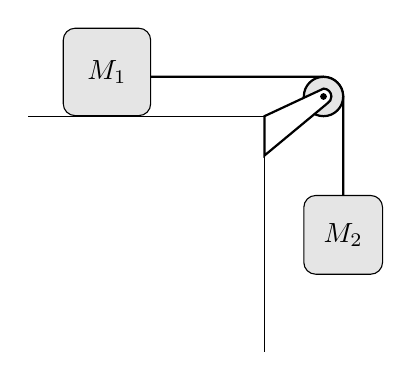
\begin{tikzpicture}
        %% Floor
        \draw (-3,0) -- (0,0) -- (0,-3);
        %% Mass
        \node[draw,fill=white!90!black,rectangle,rounded corners=1ex,minimum size=1.11cm,anchor=south] (A) at (-2,0) {$M_1$};
        \node[draw,fill=white!90!black,rectangle,rounded corners=1ex,minimum size=1.00cm,anchor=north] (B) at (1,-1) {$M_2$};
        %% Rope and Pulley
        \draw[thick] (A.south east) ++(90:0.5) -- (0.75,0.5) arc(90:0:0.25) -- (B.north);
        \draw[thick,fill=white!90!black] (0.75,0.25) circle (0.25); 
        \draw[thick,fill=white] (0,0) -- (0.75,0.35) arc (90:-60:0.1) -- (0,-0.5) -- cycle;
        \draw[fill] (0.75,0.25) circle (1pt);
    \end{tikzpicture}
    \end{center}
    The pulley (radius = \SI{0.20}{\meter}) rotates about a frictionless axle. 
    The acceleration of $M_2$ is \SI{3.5}{\meter\per\second\squared}. 
    What is the moment of inertia of the pulley?
    \begin{multicols}{2}
    \begin{choices}
        \wrongchoice{\SI{0.29}{\kilo\gram\meter\squared}}
        \wrongchoice{\SI{0.42}{\kilo\gram\meter\squared}}
      \correctchoice{\SI{0.20}{\kilo\gram\meter\squared}}
        \wrongchoice{\SI{0.62}{\kilo\gram\meter\squared}}
        \wrongchoice{\SI{0.60}{\kilo\gram\meter\squared}}
    \end{choices}
    \end{multicols}
\end{question}
}

\element{serway-mc}{
\begin{question}{serway-ch10-q15}
    A wheel (radius = \SI{0.20}{\meter}) is mounted on a frictionless, horizontal axis. 
    A light cord wrapped around the wheel supports a \SI{0.50}{\kilo\gram} object, as shown in the figure. 
    \begin{center}
    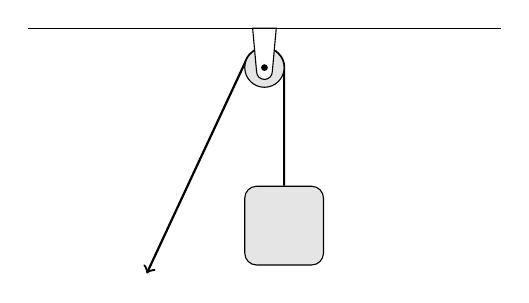
\begin{tikzpicture}
        %% Ceiling
        \draw (-3,0) -- (+3,0);
        %% Mass
        \node[draw,fill=white!90!black,rectangle,rounded corners=1ex,minimum size=1.00cm,anchor=north] (M) at (0.25,-2) {};
        %% Rope and Pulley
        \draw[thick,->] (M.north) -- (0.25,-0.50) arc(0:155:0.25) -- ++(245:3);
        \draw[fill=white!90!black] (0,-0.5) circle (0.25);
        \draw[fill=white] (-0.15,0) -- (-0.1,-0.55) arc (180:360:0.1) -- (0.15,0) -- cycle;
        \draw[fill=black] (0,-0.5) circle (1pt);
    \end{tikzpicture}
    \end{center}
    When released from rest the object falls with a downward acceleration of \SI{5.0}{\meter\per\second\squared}.
    What is the moment of inertia of the wheel?
    \begin{multicols}{2}
    \begin{choices}
        \wrongchoice{\SI{0.023}{\kilo\gram\meter\squared}}
        \wrongchoice{\SI{0.027}{\kilo\gram\meter\squared}}
        \wrongchoice{\SI{0.016}{\kilo\gram\meter\squared}}
      \correctchoice{\SI{0.019}{\kilo\gram\meter\squared}}
        \wrongchoice{\SI{0.032}{\kilo\gram\meter\squared}}
    \end{choices}
    \end{multicols}
\end{question}
}

\element{serway-mc}{
\begin{question}{serway-ch10-q16}
    A wheel (radius = \SI{0.20}{\meter}) is mounted on a frictionless, horizontal axis. 
    A light cord wrapped around the wheel supports a \SI{0.50}{\kilo\gram} object, as shown in the figure. 
    \begin{center}
    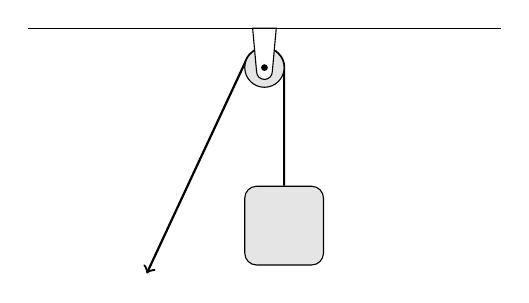
\begin{tikzpicture}
        %% Ceiling
        \draw (-3,0) -- (+3,0);
        %% Mass
        \node[draw,fill=white!90!black,rectangle,rounded corners=1ex,minimum size=1.00cm,anchor=north] (M) at (0.25,-2) {};
        %% Rope and Pulley
        \draw[thick,->] (M.north) -- (0.25,-0.50) arc(0:155:0.25) -- ++(245:3);
        \draw[fill=white!90!black] (0,-0.5) circle (0.25);
        \draw[fill=white] (-0.15,0) -- (-0.1,-0.55) arc (180:360:0.1) -- (0.15,0) -- cycle;
        \draw[fill=black] (0,-0.5) circle (1pt);
    \end{tikzpicture}
    \end{center}
    A wheel (radius = \SI{0.25}{\meter}) is mounted on a frictionless, horizontal axis. 
    The moment of inertia of the wheel about the axis is \SI{0.040}{\kilo\gram\meter\squared}.
    A light cord wrapped around the wheel supports a \SI{0.50}{\kilo\gram} object as shown in the figure. 
    The object is released from rest. 
    What is the magnitude of the acceleration of the \SI{0.50}{\kilo\gram} object?
    \begin{multicols}{3}
    \begin{choices}
        \wrongchoice{\SI{3.0}{\meter\per\second\squared}}
        \wrongchoice{\SI{3.4}{\meter\per\second\squared}}
      \correctchoice{\SI{4.3}{\meter\per\second\squared}}
        \wrongchoice{\SI{3.8}{\meter\per\second\squared}}
        \wrongchoice{\SI{2.7}{\meter\per\second\squared}}
    \end{choices}
    \end{multicols}
\end{question}
}

\element{serway-mc}{
\begin{question}{serway-ch10-q17}
    A mass $m=\SI{4.0}{\kilo\gram}$ is connected, as shown,
        by a light cord to a mass $M=\SI{6.0}{\kilo\gram}$,
    which slides on a smooth horizontal surface. 
    \begin{center}
    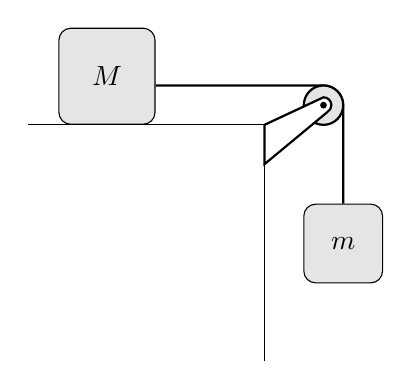
\begin{tikzpicture}
        %% Floor
        \draw (-3,0) -- (0,0) -- (0,-3);
        %% Mass
        \node[draw,fill=white!90!black,rectangle,rounded corners=1ex,minimum size=1.22cm,anchor=south] (A) at (-2,0) {$M$};
        \node[draw,fill=white!90!black,rectangle,rounded corners=1ex,minimum size=1.00cm,anchor=north] (B) at (1,-1) {$m$};
        %% Rope and Pulley
        \draw[thick] (A.south east) ++(90:0.5) -- (0.75,0.5) arc(90:0:0.25) -- (B.north);
        \draw[thick,fill=white!90!black] (0.75,0.25) circle (0.25); 
        \draw[thick,fill=white] (0,0) -- (0.75,0.35) arc (90:-60:0.1) -- (0,-0.5) -- cycle;
        \draw[fill] (0.75,0.25) circle (1pt);
    \end{tikzpicture}
    \end{center}
    The pulley rotates about a frictionless axle and has a radius $R=\SI{0.12}{\meter}$ and a moment of inertia $I=\SI{0.090}{\kilo\gram\meter\squared}$.
    The cord does not slip on the pulley. 
    What is the magnitude of the acceleration of $m$?
    \begin{multicols}{3}
    \begin{choices}
      \correctchoice{\SI{2.4}{\meter\per\second\squared}}
        \wrongchoice{\SI{2.8}{\meter\per\second\squared}}
        \wrongchoice{\SI{3.2}{\meter\per\second\squared}}
        \wrongchoice{\SI{4.2}{\meter\per\second\squared}}
        \wrongchoice{\SI{1.7}{\meter\per\second\squared}}
    \end{choices}
    \end{multicols}
\end{question}
}

\element{serway-mc}{
\begin{question}{serway-ch10-q18}
    A cylinder rotating about its axis with a constant angular acceleration of \SI{1.6}{\radian\per\second\squared} starts from rest at $t=0$.
    At the instant when it has turned through \SI{0.40}{\radian},
    what is the magnitude of the total linear acceleration of a point on the rim (radius = \SI{13}{\centi\meter})?
    \begin{multicols}{3}
    \begin{choices}
        \wrongchoice{\SI{0.31}{\meter\per\second\squared}}
      \correctchoice{\SI{0.27}{\meter\per\second\squared}}
        \wrongchoice{\SI{0.35}{\meter\per\second\squared}}
        \wrongchoice{\SI{0.39}{\meter\per\second\squared}}
        \wrongchoice{\SI{0.45}{\meter\per\second\squared}}
    \end{choices}
    \end{multicols}
\end{question}
}

\element{serway-mc}{
\begin{question}{serway-ch10-q19}
    A wheel (radius = \SI{0.20}{\meter}) starts from rest and rotates with a constant angular acceleration of \SI{2.0}{\radian\per\second\squared}. 
    At the instant when the angular velocity is equal to \SI{1.2}{\radian\per\hour},
        what is the magnitude of the total linear acceleration of a point on the rim of the wheel?
    \begin{multicols}{3}
    \begin{choices}
        \wrongchoice{\SI{0.40}{\meter\per\second\squared}}
        \wrongchoice{\SI{0.29}{\meter\per\second\squared}}
        \wrongchoice{\SI{0.69}{\meter\per\second\squared}}
      \correctchoice{\SI{0.49}{\meter\per\second\squared}}
        \wrongchoice{\SI{0.35}{\meter\per\second\squared}}
    \end{choices}
    \end{multicols}
\end{question}
}

\element{serway-mc}{
\begin{question}{serway-ch10-q20}
    A horizontal disk with a radius of \SI{10}{\centi\meter} rotates about a vertical axis through its center. 
    The disk starts from rest at $t = 0$ and has a constant angular acceleration of \SI{2.1}{\radian\per\second\squared}.
    At what value of $t$ will the radial and tangential components of the linear acceleration of a point on the rim of the disk be equal in magnitude?
    \begin{multicols}{3}
    \begin{choices}
        \wrongchoice{\SI{0.55}{\second}}
        \wrongchoice{\SI{0.63}{\second}}
      \correctchoice{\SI{0.69}{\second}}
        \wrongchoice{\SI{0.59}{\second}}
        \wrongchoice{\SI{0.47}{\second}}
    \end{choices}
    \end{multicols}
\end{question}
}

\element{serway-mc}{
\begin{question}{serway-ch10-q21}
    Two particles ($m_1=\SI{0.20}{\kilo\gram\per\meter\squared}$, $m_2=\SI{0.30}{\kilo\gram}$) are positioned at the ends of a 2.0-m
        long rod of negligible mass. 
    What is the moment of inertia of this rigid body about an axis perpendicular to the rod and through the center of mass?
    \begin{multicols}{3}
    \begin{choices}
      \correctchoice{\SI{0.48}{\kilo\gram\meter\squared}}
        \wrongchoice{\SI{0.50}{\kilo\gram\meter\squared}}
        \wrongchoice{\SI{1.2}{\kilo\gram\meter\squared}}
        \wrongchoice{\SI{0.80}{\kilo\gram\meter\squared}}
        \wrongchoice{\SI{0.70}{\kilo\gram\meter\squared}}
    \end{choices}
    \end{multicols}
\end{question}
}

\element{serway-mc}{
\begin{question}{serway-ch10-q22}
    Four identical particles (mass of each = \SI{0.24}{\kilo\gram}) are placed at the vertices of a rectangle $\left(\SI{2.0}{\meter}\times\SI{3.0}{\meter}\right)$ and held in those positions by four light rods which form the sides of the rectangle. 
    What is the moment of inertia of this rigid body about an axis that passes through the center of mass of the body and is parallel to the shorter sides of the rectangle?
    \begin{multicols}{3}
    \begin{choices}
        \wrongchoice{\SI{2.4}{\kilo\gram\meter\squared}}
      \correctchoice{\SI{2.2}{\kilo\gram\meter\squared}}
        \wrongchoice{\SI{1.9}{\kilo\gram\meter\squared}}
        \wrongchoice{\SI{2.7}{\kilo\gram\meter\squared}}
        \wrongchoice{\SI{8.6}{\kilo\gram\meter\squared}}
    \end{choices}
    \end{multicols}
\end{question}
}

\element{serway-mc}{
\begin{question}{serway-ch10-q23}
    Four identical particles (mass of each = \SI{0.40}{\kilo\gram}) are placed at the vertices of a rectangle $\left(\SI{2.5}{\meter}\times\SI{4.0}{\meter}\right)$ and held in those positions by four light rods which form the sides of the rectangle. 
    What is the moment of inertia of this rigid body about an axis that passes through the mid-points of the shorter sides and is parallel to the longer sides?
    \begin{multicols}{3}
    \begin{choices}
        \wrongchoice{\SI{2.2}{\kilo\gram\meter\squared}}
        \wrongchoice{\SI{2.8}{\kilo\gram\meter\squared}}
      \correctchoice{\SI{2.5}{\kilo\gram\meter\squared}}
        \wrongchoice{\SI{3.1}{\kilo\gram\meter\squared}}
        \wrongchoice{\SI{1.6}{\kilo\gram\meter\squared}}
    \end{choices}
    \end{multicols}
\end{question}
}

\element{serway-mc}{
\begin{question}{serway-ch10-q24}
    Four identical particles (mass of each = \SI{0.40}{\kilo\gram}) are placed at the vertices of a rectangle $\left(\SI{2.0}{\meter}\times\SI{3.0}{\meter}\right)$ and held in those positions by four light rods which form the sides of the rectangle. 
    What is the moment of inertia of this rigid body about an axis that passes through the mid-points of the longer sides and is parallel to the shorter sides?
    \begin{multicols}{3}
    \begin{choices}
        \wrongchoice{\SI{2.7}{\kilo\gram\meter\squared}}
      \correctchoice{\SI{3.6}{\kilo\gram\meter\squared}}
        \wrongchoice{\SI{3.1}{\kilo\gram\meter\squared}}
        \wrongchoice{\SI{4.1}{\kilo\gram\meter\squared}}
        \wrongchoice{\SI{1.6}{\kilo\gram\meter\squared}}
    \end{choices}
    \end{multicols}
\end{question}
}

\element{serway-mc}{
\begin{question}{serway-ch10-q25}
    The rigid object shown is rotated about an axis perpendicular to the paper and through point $P$.
    The total kinetic energy of the object as it rotates is equal to \SI{1.4}{\joule}.
    \begin{center}
    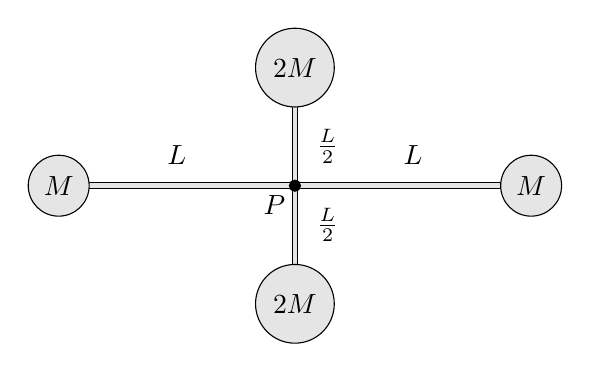
\begin{tikzpicture}
        %% Bars
        \draw[draw,fill=white!90!black] (-3,-1pt) rectangle (+3,+1pt);
        \draw[draw,fill=white!90!black] (-1pt,-1.5) rectangle (+1pt,+1.5);
        \node[anchor=south,yshift=1ex] at (-1.5,0) {$L$};
        \node[anchor=south,yshift=1ex] at (+1.5,0) {$L$};
        \node[anchor=west,xshift=1ex] at (0,0.50) {$\frac{L}{2}$};
        \node[anchor=west,xshift=1ex] at (0,-0.50) {$\frac{L}{2}$};
        %% Balls
        \node[draw,fill=white!90!black,minimum size=0.707cm,circle] (A) at (-3.0,0) {$M$};
        \node[draw,fill=white!90!black,minimum size=0.707cm,circle] (B) at (+3.0,0) {$M$};
        \node[draw,fill=white!90!black,minimum size=1cm,circle] (C) at (0,+1.5) {$2M$};
        \node[draw,fill=white!90!black,minimum size=1cm,circle] (C) at (0,-1.5) {$2M$};
        %% Labels
        \draw[fill] (0,0) circle (2pt) node[anchor=north east] {$P$};
    \end{tikzpicture}
    \end{center}
    If $M=\SI{1.3}{\kilo\gram}$ and $L=\SI{0.50}{\meter}$,
        what is the angular velocity of the object? 
    Neglect the mass of the connecting rods and treat the masses as particles.
    \begin{multicols}{3}
    \begin{choices}
        \wrongchoice{\SI{1.3}{\radian\per\second}}
        \wrongchoice{\SI{1.5}{\radian\per\second}}
      \correctchoice{\SI{1.7}{\radian\per\second}}
        \wrongchoice{\SI{1.2}{\radian\per\second}}
        \wrongchoice{\SI{2.1}{\radian\per\second}}
    \end{choices}
    \end{multicols}
\end{question}
}

\element{serway-mc}{
\begin{question}{serway-ch10-q26}
    If $M=\SI{0.50}{\kilo\gram}$, $L=\SI{1.2}{\meter}$,
        and the mass of each connecting rod shown is negligible,
    \begin{center}
    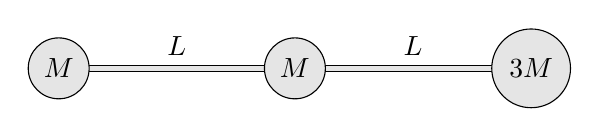
\begin{tikzpicture}
        %% Bars
        \draw[draw,fill=white!90!black] (-3,-1pt) rectangle (+3,+1pt);
        \node[anchor=south,yshift=1pt] at (-1.5,0) {$L$};
        \node[anchor=south,yshift=1pt] at (+1.5,0) {$L$};
        %% Balls
        \node[draw,fill=white!90!black,minimum size=0.57cm,circle,anchor=center] (A) at (-3,0) {$M$};
        \node[draw,fill=white!90!black,minimum size=0.57cm,circle,anchor=center] (B) at (+0,0) {$M$};
        \node[draw,fill=white!90!black,minimum size=1.00cm,circle,anchor=center] (C) at (+3,0) {$3M$};
    \end{tikzpicture}
    \end{center}
        what is the moment of inertia about an axis perpendicular to the paper through the center of mass?
    Treat the mass as particles.
    \begin{multicols}{3}
    \begin{choices}
        \wrongchoice{\SI{3.7}{\kilo\gram\meter\squared}}
        \wrongchoice{\SI{2.8}{\kilo\gram\meter\squared}}
        \wrongchoice{\SI{3.2}{\kilo\gram\meter\squared}}
      \correctchoice{\SI{2.3}{\kilo\gram\meter\squared}}
        \wrongchoice{\SI{3.9}{\kilo\gram\meter\squared}}
    \end{choices}
    \end{multicols}
\end{question}
}

\element{serway-mc}{
\begin{question}{serway-ch10-q27}
    Three particles, each of which has a mass of \SI{80}{\gram},
        are positioned at the vertices of an equilateral triangle with sides of length \SI{60}{\centi\meter}.
    The particles are connected by rods of negligible mass. 
    What is the moment of inertia of this rigid body about an axis that is parallel to one side of the triangle and passes through the respective midpoints of the other two sides?
    \begin{multicols}{2}
    \begin{choices}
        \wrongchoice{\SI{0.018}{\kilo\gram\meter\squared}}
        \wrongchoice{\SI{0.020}{\kilo\gram\meter\squared}}
      \correctchoice{\SI{0.016}{\kilo\gram\meter\squared}}
        \wrongchoice{\SI{0.022}{\kilo\gram\meter\squared}}
        \wrongchoice{\SI{0.032}{\kilo\gram\meter\squared}}
    \end{choices}
    \end{multicols}
\end{question}
}

\element{serway-mc}{
\begin{question}{serway-ch10-q28}
    A uniform rod (mass = \SI{2.0}{\kilo\gram}, length = \SI{0.60}{\meter}) is free to rotate about a frictionless pivot at one end. 
    The rod is released from rest in the horizontal position. 
    What is the magnitude of the angular acceleration of the rod at the instant it is \ang{60} below the horizontal?
    \begin{multicols}{3}
    \begin{choices}
        \wrongchoice{\SI{15}{\radian\per\second\squared}}
      \correctchoice{\SI{12}{\radian\per\second\squared}}
        \wrongchoice{\SI{18}{\radian\per\second\squared}}
        \wrongchoice{\SI{29}{\radian\per\second\squared}}
        \wrongchoice{\SI{23}{\radian\per\second\squared}}
    \end{choices}
    \end{multicols}
\end{question}
}

\element{serway-mc}{
\begin{question}{serway-ch10-q29}
    Particles (mass of each = \SI{0.20}{\kilo\gram}) are placed at the \SI{40}{\centi\meter} and \SI{100}{\centi\meter} marks of a meter stick of negligible mass. 
    This rigid body is free to rotate about a frictionless pivot at the \SI{0}{\centi\meter} end. 
    The body is released from rest in the horizontal position.
    What is the initial angular acceleration of the body?
    \begin{multicols}{3}
    \begin{choices}
      \correctchoice{\SI{12}{\radian\per\second\squared}}
        \wrongchoice{\SI{5.9}{\radian\per\second\squared}}
        \wrongchoice{\SI{8.4}{\radian\per\second\squared}}
        \wrongchoice{\SI{5.4}{\radian\per\second\squared}}
        \wrongchoice{\SI{17}{\radian\per\second\squared}}
    \end{choices}
    \end{multicols}
\end{question}
}

\element{serway-mc}{
\begin{question}{serway-ch10-q30}
    Particles (mass of each = \SI{0.40}{\kilo\gram}) are placed at the \SI{60}{\centi\meter} and \SI{100}{\centi\meter} marks of a meter stick of negligible mass. 
    This rigid body is free to rotate about a frictionless pivot at the \SI{0}{\centi\meter} end. 
    The body is released from rest in the horizontal position.
    What is the magnitude of the initial linear acceleration of the end of the body opposite the pivot?
    \begin{multicols}{3}
    \begin{choices}
        \wrongchoice{\SI{15}{\meter\per\second\squared}}
        \wrongchoice{\SI{9.8}{\meter\per\second\squared}}
        \wrongchoice{\SI{5.8}{\meter\per\second\squared}}
      \correctchoice{\SI{12}{\meter\per\second\squared}}
        \wrongchoice{\SI{4.7}{\meter\per\second\squared}}
    \end{choices}
    \end{multicols}
\end{question}
}

\element{serway-mc}{
\begin{question}{serway-ch10-q31}
    A wheel (radius = \SI{12}{\centi\meter}) is mounted on a frictionless, horizontal axle that is perpendicular to the wheel and passes through the center of mass of the wheel.
    A light cord wrapped around the wheel supports a \SI{0.40}{\kilo\gram} object. 
    If released from rest with the string taut,
        the object is observed to fall with a downward acceleration of \SI{3.0}{\meter\per\second\squared}. 
    What is the moment of inertia (of the wheel) about the given axle?
    \begin{multicols}{2}
    \begin{choices}
        \wrongchoice{\SI{0.023}{\kilo\gram\meter\squared}}
      \correctchoice{\SI{0.013}{\kilo\gram\meter\squared}}
        \wrongchoice{\SI{0.020}{\kilo\gram\meter\squared}}
        \wrongchoice{\SI{0.016}{\kilo\gram\meter\squared}}
        \wrongchoice{\SI{0.035}{\kilo\gram\meter\squared}}
    \end{choices}
    \end{multicols}
\end{question}
}

\element{serway-mc}{
\begin{question}{serway-ch10-q32}
    A uniform rod is \SI{2.0}{\meter} long. 
    The rod is pivoted about a horizontal, frictionless pin through one end. 
    The rod is released from rest at an angle of \ang{30} above the horizontal.
    What is the angular acceleration of the rod at the instant it is released?
    \begin{multicols}{3}
    \begin{choices}
        \wrongchoice{\SI{4.7}{\radian\per\second\squared}}
        \wrongchoice{\SI{6.9}{\radian\per\second\squared}}
      \correctchoice{\SI{6.4}{\radian\per\second\squared}}
        \wrongchoice{\SI{5.6}{\radian\per\second\squared}}
        \wrongchoice{\SI{4.2}{\radian\per\second\squared}}
    \end{choices}
    \end{multicols}
\end{question}
}

\element{serway-mc}{
\begin{question}{serway-ch10-q33}
    A uniform rod is \SI{2.0}{\meter} long. 
    The rod is pivoted about a horizontal, frictionless pin through one end. 
    The rod is released from rest at the horizontal position.
    What is the angular acceleration of the rod at the instant the rod makes an angle of \ang{70} with the horizontal?
    \begin{multicols}{3}
    \begin{choices}
        \wrongchoice{\SI{3.7}{\radian\per\second\squared}}
        \wrongchoice{\SI{1.3}{\radian\per\second\squared}}
      \correctchoice{\SI{2.5}{\radian\per\second\squared}}
        \wrongchoice{\SI{4.9}{\radian\per\second\squared}}
        \wrongchoice{\SI{1.9}{\radian\per\second\squared}}
    \end{choices}
    \end{multicols}
\end{question}
}

\element{serway-mc}{
\begin{question}{serway-ch10-q34}
    A uniform rod of mass $M=\SI{1.2}{\kilo\gram}$ and length $L=\SI{0.80}{\meter}$,
        lying on a frictionless horizontal plane,
        is free to pivot about a vertical axis through one end, as shown.
    \begin{center}
    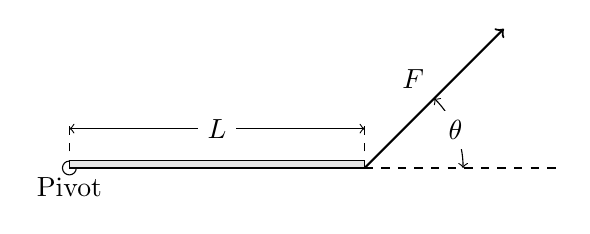
\begin{tikzpicture}[scale=1.25]
        %% Uniform Rod
        \draw (0,0) circle (2pt) node[anchor=north] {Pivot};
        \draw[fill=white!90!black] (0,0) rectangle (3,0.5ex);
        %% Label
        \draw[dashed] (0,0) -- ++(90:0.5);
        \draw[dashed] (3,0) -- ++(90:0.5);
        \draw[<->] (0,0.4) -- (3,0.4) node[anchor=center,fill=white,pos=0.5] {$L$};
        %% Vector
        \draw[thick,->] (3,0) -- ++(45:2) node[pos=0.5,anchor=south east] {$F$};
        \draw[dashed] (3,0) -- ++(0:2);
        \draw[<->] (4,0) arc (0:45:1) node[anchor=center,pos=0.5,fill=white] {$\theta$};
    \end{tikzpicture}
    \end{center}
    The moment of inertia of the rod about this axis is given by $ML^2$. 
    If a force ($F=\SI{5.0}{\newton}$, $\theta=\ang{40}$) acts as shown,
        what is the resulting angular acceleration about the pivot point?
    \begin{multicols}{3}
    \begin{choices}
        \wrongchoice{\SI{16}{\radian\per\second\squared}}
        \wrongchoice{\SI{12}{\radian\per\second\squared}}
        \wrongchoice{\SI{14}{\radian\per\second\squared}}
      \correctchoice{\SI{10}{\radian\per\second\squared}}
        \wrongchoice{\SI{33}{\radian\per\second\squared}}
    \end{choices}
    \end{multicols}
\end{question}
}

\element{serway-mc}{
\begin{question}{serway-ch10-q35}
    A uniform meter stick is pivoted to rotate about a horizontal axis through the \SI{25}{\centi\meter} mark on the stick. 
    The stick is released from rest in a horizontal position.
    The moment of inertia of a uniform rod about an axis perpendicular to the rod and through the center of mass of the rod is given by $\dfrac{1}{12}ML^2$. 
    Determine the magnitude of the initial angular acceleration of the stick.
    \begin{multicols}{3}
    \begin{choices}
      \correctchoice{\SI{17}{\radian\per\second\squared}}
        \wrongchoice{\SI{13}{\radian\per\second\squared}}
        \wrongchoice{\SI{15}{\radian\per\second\squared}}
        \wrongchoice{\SI{19}{\radian\per\second\squared}}
        \wrongchoice{\SI{23}{\radian\per\second\squared}}
    \end{choices}
    \end{multicols}
\end{question}
}

\element{serway-mc}{
\begin{question}{serway-ch10-q36}
    A uniform rod (length = \SI{2.0}{\meter}) is mounted to rotate freely about a horizontal axis that is perpendicular to the rod and that passes through the rod at a point \SI{0.50}{\meter} from one end of the rod. 
    If the rod is released from rest in a horizontal position,
        what is the angular speed of the rod as it rotates through its lowest position?
    \begin{multicols}{3}
    \begin{choices}
        \wrongchoice{\SI{3.5}{\radian\per\second}}
        \wrongchoice{\SI{3.8}{\radian\per\second}}
      \correctchoice{\SI{4.1}{\radian\per\second}}
        \wrongchoice{\SI{2.0}{\radian\per\second}}
        \wrongchoice{\SI{5.6}{\radian\per\second}}
    \end{choices}
    \end{multicols}
\end{question}
}

\element{serway-mc}{
\begin{question}{serway-ch10-q37}
    Identical particles are placed at the \SI{50}{\centi\meter} and \SI{80}{\centi\meter} marks on a meter stick of negligible mass. 
    This rigid body is then mounted so as to rotate freely about a pivot at the \SI{0}{\centi\meter} mark on the meter stick. 
    If this body is released from rest in a horizontal position,
        what is the angular speed of the meter stick as it swings through its lowest position?
    \begin{multicols}{3}
    \begin{choices}
        \wrongchoice{\SI{4.2}{\radian\per\second}}
      \correctchoice{\SI{5.4}{\radian\per\second}}
        \wrongchoice{\SI{4.6}{\radian\per\second}}
        \wrongchoice{\SI{5.0}{\radian\per\second}}
        \wrongchoice{\SI{1.7}{\radian\per\second}}
    \end{choices}
    \end{multicols}
\end{question}
}

\element{serway-mc}{
\begin{question}{serway-ch10-q38}
    A uniform rod (mass = \SI{1.5}{\kilo\gram}) is \SI{2.0}{\meter} long. 
    The rod is pivoted about a horizontal,
        frictionless pin through one end. 
    The rod is released from rest in a horizontal position. 
    What is the angular speed of the rod when the rod makes an angle of \ang{30} with the horizontal?
    (The moment of inertia of the rod about the pin is \SI{2.0}{\kilo\gram\meter\squared}).
    \begin{multicols}{3}
    \begin{choices}
        \wrongchoice{\SI{2.2}{\radian\per\second}}
        \wrongchoice{\SI{3.6}{\radian\per\second}}
      \correctchoice{\SI{2.7}{\radian\per\second}}
        \wrongchoice{\SI{3.1}{\radian\per\second}}
        \wrongchoice{\SI{1.8}{\radian\per\second}}
    \end{choices}
    \end{multicols}
\end{question}
}

\element{serway-mc}{
\begin{question}{serway-ch10-q39}
    A uniform rod is \SI{3.0}{\meter} long. 
    The rod is pivoted about a horizontal,
        frictionless pin through one end. 
    The rod is released from rest at an angle of \ang{27} above the horizontal.
    What is the angular speed of the rod as it passes through the horizontal position?
    \begin{multicols}{3}
    \begin{choices}
        \wrongchoice{\SI{3.0}{\radian\per\second}}
        \wrongchoice{\SI{2.8}{\radian\per\second}}
      \correctchoice{\SI{2.1}{\radian\per\second}}
        \wrongchoice{\SI{2.5}{\radian\per\second}}
        \wrongchoice{\SI{3.4}{\radian\per\second}}
    \end{choices}
    \end{multicols}
\end{question}
}

\element{serway-mc}{
\begin{question}{serway-ch10-q40}
    A uniform rod of length $\left(L=\SI{2.0}{\meter}\right)$ and mass $\left(M=\SI{1.5}{\kilo\gram}\right)$ is pivoted about a horizontal frictionless pin through one end. 
    The rod is released from rest at an angle of \ang{30} below the horizontal. 
    What is the angular speed of the rod when it passes through the vertical position?
    (The moment of inertia of the rod about the pin is \SI{2.0}{\kilo\gram\meter\squared}.)
    \begin{multicols}{3}
    \begin{choices}
        \wrongchoice{\SI{3.5}{\radian\per\second}}
      \correctchoice{\SI{2.7}{\radian\per\second}}
        \wrongchoice{\SI{3.1}{\radian\per\second}}
        \wrongchoice{\SI{2.3}{\radian\per\second}}
        \wrongchoice{\SI{1.6}{\radian\per\second}}
    \end{choices}
    \end{multicols}
\end{question}
}

\element{serway-mc}{
\begin{question}{serway-ch10-q41}
    A nonuniform \SI{2.0}{\kilo\gram} rod is \SI{2.0}{\meter} long. 
    The rod is mounted to rotate freely about a horizontal axis perpendicular to the rod that passes through one end of the rod.
    The moment of inertia of the rod about this axis is \SI{4.0}{\kilo\gram\meter\squared}. 
    The center of mass of the rod is \SI{1.2}{\meter} from the axis. 
    If the rod is released from rest in the horizontal position,
        what is its angular speed as it swings through the vertical position?
    \begin{multicols}{3}
    \begin{choices}
      \correctchoice{\SI{3.4}{\radian\per\second}}
        \wrongchoice{\SI{4.4}{\radian\per\second}}
        \wrongchoice{\SI{4.3}{\radian\per\second}}
        \wrongchoice{\SI{5.8}{\radian\per\second}}
        \wrongchoice{\SI{6.8}{\radian\per\second}}
    \end{choices}
    \end{multicols}
\end{question}
}

\element{serway-mc}{
\begin{question}{serway-ch10-q42}
    The rigid body shown rotates about an axis through its center of mass and perpendicular to the paper. 
    \begin{center}
    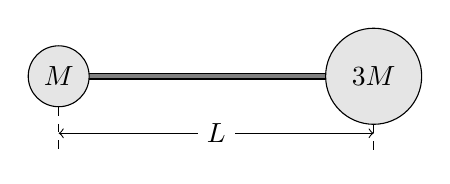
\begin{tikzpicture}
        %% Rod
        \draw[fill=white!50!black] (-2cm,-1pt) rectangle (+2cm,+1pt);
        %% Balls
        \node[draw,circle,fill=white!90!black,minimum size=0.71cm] (A) at (-2,0) {$M$};
        \node[draw,circle,fill=white!90!black,minimum size=1.22cm] (B) at (+2,0) {$3M$};
        %% Labels
        \draw[dashed] (A.south) -- (-2,-1);
        \draw[dashed] (B.south) -- (+2,-1);
        \draw[<->] (A.south) ++ (270:0.33) -- ++ (0:4) node[pos=0.5,anchor=center,fill=white] {$L$};
    \end{tikzpicture}
    \end{center}
    If $M=\SI{2.0}{\kilo\gram}$ and $L=\SI{80}{\centi\meter}$,
        what is the kinetic energy of this object when its angular speed about this axis is equal to \SI{5.0}{\radian\per\second}?
    Neglect the mass of the connecting rod and treat the masses as particles.
    \begin{multicols}{3}
    \begin{choices}
        \wrongchoice{\SI{18}{\joule}}
        \wrongchoice{\SI{15}{\joule}}
      \correctchoice{\SI{12}{\joule}}
        \wrongchoice{\SI{23}{\joule}}
        \wrongchoice{\SI{26}{\joule}}
    \end{choices}
    \end{multicols}
\end{question}
}

\element{serway-mc}{
\begin{question}{serway-ch10-q43}
    The rigid body shown is rotated about an axis perpendicular to the paper and through the point $P$. 
    \begin{center}
    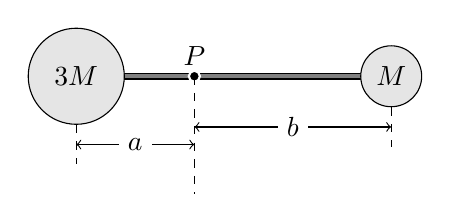
\begin{tikzpicture}
        %% Rod
        \draw[fill=white!50!black] (-2,-1pt) rectangle (+2,+1pt);
        %% Balls
        \node[draw,circle,fill=white!90!black,minimum size=1.22cm] (A) at (-2,0) {$3M$};
        \node[draw,circle,fill=white!90!black,minimum size=0.71cm] (B) at (+2,0) {$M$};
        %% Pivot
        \draw[draw=white,thick,fill=black] (-0.5,0) circle (2pt) node[anchor=south] {$P$};
        \draw[dashed] (-0.5,0) -- ++(270:1.5);
        %% Labels
        \draw[dashed] (A.south) -- ++(270:0.5);
        \draw[dashed] (B.south) -- ++(270:0.5);
        \draw[<->] (A.south) ++ (270:0.25) -- ++(0:1.5) node[pos=0.5,anchor=center,fill=white] {$a$};
        \draw[<->] (B.south) ++ (270:0.25) -- ++(180:2.5) node[pos=0.5,anchor=center,fill=white] {$b$};
    \end{tikzpicture}
    \end{center}
    If $M=\SI{0.40}{\kilo\gram}$, $a=\SI{30}{\centi\meter}$, and $b=\SI{50}{\centi\meter}$,
        how much work is required to take the body from rest to an angular speed of \SI{5.0}{\radian\per\second}? 
    Neglect the mass of the connecting rods and treat the masses as particles.
    \begin{multicols}{3}
    \begin{choices}
        \wrongchoice{\SI{2.9}{\joule}}
      \correctchoice{\SI{2.6}{\joule}}
        \wrongchoice{\SI{3.1}{\joule}}
        \wrongchoice{\SI{3.4}{\joule}}
        \wrongchoice{\SI{1.6}{\joule}}
    \end{choices}
    \end{multicols}
\end{question}
}

\element{serway-mc}{
\begin{question}{serway-ch10-q44}
    A uniform rod (length = \SI{2.4}{\meter}) of negligible mass has a \SI{1.0}{\kilo\gram} point mass attached to one end and a \SI{2.0}{\kilo\gram} point mass attached to the other end. 
    The rod is mounted to rotate freely about a horizontal axis that is perpendicular to the rod and that passes through a point \SI{1.0}{\meter} from the \SI{2.0}{\kilo\gram} mass. 
    The rod is released from rest when it is horizontal. 
    What is the angular velocity of the rod at the instant the \SI{2.0}{\kilo\gram} mass passes through its low point?
    \begin{multicols}{3}
    \begin{choices}
      \correctchoice{\SI{1.7}{\radian\per\second}}
        \wrongchoice{\SI{2.2}{\radian\per\second}}
        \wrongchoice{\SI{2.0}{\radian\per\second}}
        \wrongchoice{\SI{1.5}{\radian\per\second}}
        \wrongchoice{\SI{3.1}{\radian\per\second}}
    \end{choices}
    \end{multicols}
\end{question}
}

\element{serway-mc}{
\begin{question}{serway-ch10-q45}
    A campus bird spots a member of an opposing football team in an amusement park.
    The football player is on a ride where he goes around at angular velocity $\omega$ at distance $R$ from the center. 
    The bird flies in a horizontal circle above him. 
    Will a dropping the bird releases while flying directly above the person's head hit him?
    \begin{choices}
        \wrongchoice{Yes, because it falls straight down.}
        \wrongchoice{Yes, because it maintains the acceleration of the bird as it falls.}
        \wrongchoice{No, because it falls straight down and will land behind the person.}
        \wrongchoice{Yes, because it mainatins the angular velocity of the bird as it falls.}
      \correctchoice{No, because it maintains the tangential velocity the bird had at the instant it started falling.}
    \end{choices}
\end{question}
}

\element{serway-mc}{
\begin{question}{serway-ch10-q46}
    Two people are on a ride where the inside cars rotate at constant angular velocity three times the constant angular velocity of the outer cars. 
    If the two cars are in line at $t=0$,
        and moving at $3\omega$ and $\omega$ respectively,
        at what time will they next pass each other?
    \begin{multicols}{3}
    \begin{choices}
        \wrongchoice{$t=0$}
        \wrongchoice{$t=\dfrac{\pi}{2\omega}$}
      \correctchoice{$t=\dfrac{\pi}{\omega}$}
        \wrongchoice{$t=\dfrac{2\pi}{\omega}$}
        \wrongchoice{$t=\dfrac{3\pi}{\omega}$}
    \end{choices}
    \end{multicols}
\end{question}
}

\element{serway-mc}{
\begin{question}{serway-ch10-q47}
    The figure below shows a graph of angular velocity as a function of time for a car driving around a circular track.
    \begin{center}
    \begin{tikzpicture}
        \begin{axis}[
            axis y line=left,
            axis x line=middle,
            axis line style={->},
            xlabel={$t$},
            x label style={
                at={(current axis.right of origin)},
                anchor=west,
            },
            x unit=\si{\second},
            xtick={4,8,12,16},
            ylabel={$\omega$},
            y unit=\si{\radian\per\second},
            ytick={-10,-5,0,5,10},
            grid=major,
            xmin=0,xmax=17,
            ymin=-11,ymax=11,
            width=0.8\columnwidth,
            height=0.5\columnwidth,
        ]
        \addplot[line width=1pt,mark=\empty] coordinates { (0,0) (4,10) (8,10) (12,-10) (14,-10) (16,0) };
        \end{axis}
    \end{tikzpicture}
    \end{center}
    Through how many radians does the car travel in the first 10 minutes?
    \begin{multicols}{3}
    \begin{choices}
        \wrongchoice{\SI{30}{\radian}}
        \wrongchoice{\SI{50}{\radian}}
      \correctchoice{\SI{70}{\radian}}
        \wrongchoice{\SI{90}{\radian}}
        \wrongchoice{\SI{100}{\radian}}
    \end{choices}
    \end{multicols}
\end{question}
}

\element{serway-mc}{
\begin{question}{serway-ch10-q48}
    The graphs below show angular velocity as a function of time. 
    In which one is the magnitude of the angular acceleration constantly decreasing?
    \begin{multicols}{2}
    \begin{choices}
        \AMCboxDimensions{down=-1.5em}
        \wrongchoice{
            \begin{tikzpicture}
                \begin{axis}[
                    axis y line=left,
                    axis x line=middle,
                    axis line style={->},
                    xlabel={$t$},
                    x label style={
                        at={(current axis.right of origin)},
                        anchor=west,
                    },
                    xtick=\empty,
                    ylabel={$\omega$},
                    %y label style={
                    %    at={(current axis.above origin)},
                    %    anchor=south,
                    %    rotate=270,
                    %},
                    ytick=\empty,
                    grid=major,
                    xmin=0,xmax=11,
                    ymin=-11,ymax=11,
                    width=0.98\columnwidth,
                    %height=0.618\columnwidth,
                ]
                \addplot[line width=1pt,mark=\empty,domain=0:10] {8};
                \end{axis}
            \end{tikzpicture}
        }
        \wrongchoice{
            \begin{tikzpicture}
                \begin{axis}[
                    axis y line=left,
                    axis x line=middle,
                    axis line style={->},
                    xlabel={$t$},
                    x label style={
                        at={(current axis.right of origin)},
                        anchor=west,
                    },
                    xtick=\empty,
                    ylabel={$\omega$},
                    %y label style={
                    %    at={(current axis.above origin)},
                    %    anchor=south,
                    %    rotate=270,
                    %},
                    ytick=\empty,
                    grid=major,
                    xmin=0,xmax=11,
                    ymin=-11,ymax=11,
                    width=0.98\columnwidth,
                    %height=0.618\columnwidth,
                ]
                \addplot[line width=1pt,mark=\empty,domain=0:10] {2+0.6*x};
                \end{axis}
            \end{tikzpicture}
        }
        \wrongchoice{
            \begin{tikzpicture}
                \begin{axis}[
                    axis y line=left,
                    axis x line=middle,
                    axis line style={->},
                    xlabel={$t$},
                    x label style={
                        at={(current axis.right of origin)},
                        anchor=west,
                    },
                    xtick=\empty,
                    ylabel={$\omega$},
                    %y label style={
                    %    at={(current axis.above origin)},
                    %    anchor=south,
                    %    rotate=270,
                    %},
                    ytick=\empty,
                    grid=major,
                    xmin=0,xmax=11,
                    ymin=-11,ymax=11,
                    width=0.98\columnwidth,
                    %height=0.618\columnwidth,
                ]
                \addplot[line width=1pt,mark=\empty,domain=0:10] {-2-0.6*x};
                \end{axis}
            \end{tikzpicture}
        }
        \wrongchoice{
            \begin{tikzpicture}
                \begin{axis}[
                    axis y line=left,
                    axis x line=middle,
                    axis line style={->},
                    xlabel={$t$},
                    x label style={
                        at={(current axis.right of origin)},
                        anchor=west,
                    },
                    xtick=\empty,
                    ylabel={$\omega$},
                    %y label style={
                    %    at={(current axis.above origin)},
                    %    anchor=south,
                    %    rotate=270,
                    %},
                    ytick=\empty,
                    grid=major,
                    xmin=0,xmax=11,
                    ymin=-11,ymax=11,
                    width=0.98\columnwidth,
                    %height=0.618\columnwidth,
                ]
                \addplot[line width=1pt,mark=\empty,domain=0:10] {-0.1*x*x};
                \end{axis}
            \end{tikzpicture}
        }
        %% ANS is E
        \correctchoice{
            \begin{tikzpicture}
                \begin{axis}[
                    axis y line=left,
                    axis x line=middle,
                    axis line style={->},
                    xlabel={$t$},
                    x label style={
                        at={(current axis.right of origin)},
                        anchor=west,
                    },
                    xtick=\empty,
                    ylabel={$\omega$},
                    %y label style={
                    %    at={(current axis.above origin)},
                    %    anchor=south,
                    %    rotate=270,
                    %},
                    ytick=\empty,
                    grid=major,
                    xmin=0,xmax=11,
                    ymin=-11,ymax=11,
                    width=0.98\columnwidth,
                    %height=0.618\columnwidth,
                ]
                \addplot[line width=1pt,mark=\empty,domain=0:10] {10 - 0.1*(x-10)*(x-10)};
                \end{axis}
            \end{tikzpicture}
        }
    \end{choices}
    \end{multicols}
\end{question}
}

\element{serway-mc}{
\begin{question}{serway-ch10-q49}
    You throw a Frisbee of mass $m$ and radius $r$ so that it is spinning about a horizontal axis perpendicular to the plane of the Frisbee. 
    Ignoring air resistance,
        the torque exerted about its center of mass by gravity is:
    \begin{choices}
      \correctchoice{zero}
        \wrongchoice{$mgr$}
        \wrongchoice{$2mgr$}
        \wrongchoice{a function of the angular velocity}
        \wrongchoice{small at first,
            then increasing as the Frisbee loses the torque given it by your hand}
    \end{choices}
\end{question}
}

\element{serway-mc}{
\begin{question}{serway-ch10-q50}
    Two forces of magnitude \SI{50}{\newton},
        as shown in the figure below,
        act on a cylinder of radius \SI{4}{\meter} and mass \SI{6.25}{\kilo\gram}.
    \begin{center}
    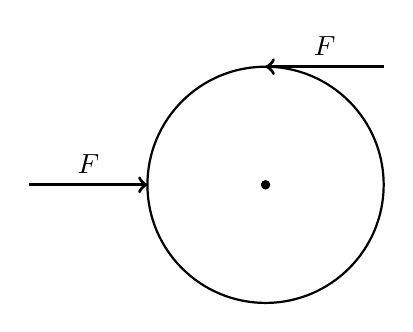
\begin{tikzpicture}[scale=0.75]
        \draw[thick] (0,0) circle (2);
        \draw[fill] (0,0) circle (2pt);
        \draw[very thick,<-] (0,2) -- ++ (0:2) node[anchor=south,pos=0.5] {$F$};
        \draw[very thick,<-] (-2,0) -- ++ (180:2) node[anchor=south,pos=0.5] {$F$};
    \end{tikzpicture}
    \end{center}
    The cylinder, which is initially at rest,
        sits on a frictionless surface. 
    After one second,
        the velocity and angular velocity of the cylinder are respectively:
    %in \si{\meter\per\second} and \si{\radian\per\second} are respectively:
    \begin{choices}
        \wrongchoice{$v=\SI{0}{\radian\per\second}$;\hspace{1em} $\omega=\SI{0}{\radian\per\second\squared}$}
      \correctchoice{$v=\SI{0}{\radian\per\second}$;\hspace{1em} $\omega=\SI{4}{\radian\per\second\squared}$}
        \wrongchoice{$v=\SI{0}{\radian\per\second}$;\hspace{1em} $\omega=\SI{8}{\radian\per\second\squared}$}
        \wrongchoice{$v=\SI{8}{\radian\per\second}$;\hspace{1em} $\omega=\SI{8}{\radian\per\second\squared}$}
        \wrongchoice{$v=\SI{16}{\radian\per\second}$;\hspace{1em} $\omega=\SI{8}{\radian\per\second\squared}$}
    \end{choices}
\end{question}
}

\element{serway-mc}{
\begin{question}{serway-ch10-q51}
    Two cylinders made of the same material roll down a plane inclined at an angle $\theta$ with the horizontal. 
    Each travels the same distance. 
    The radius of cylinder $B$ is twice the radius of cylinder $A$. 
    In what order do they reach the bottom?
    \begin{choices}
        \wrongchoice{$A$ reaches the bottom first because it has the greater acceleration.}
        \wrongchoice{$A$ reaches the bottom first because it has a smaller moment of inertia.}
        \wrongchoice{$B$ reaches the bottom first because is experiences a larger torque.}
        \wrongchoice{$B$ reaches the bottom first because it travels a larger distance in one rotation.}
      \correctchoice{They both reach the bottom at the same time, because each has the same linear acceleration.}
    \end{choices}
\end{question}
}

\newcommand{\serwayChTenQFiftyTwo}{
\begin{tikzpicture}
    \begin{axis}[
        axis y line=left,
        axis x line=middle,
        axis line style={->},
        xlabel={$t$},
        x label style={
            at={(current axis.right of origin)},
            anchor=west,
        },
        x unit=\si{\minute},
        xtick={0,4,8,12,16},
        minor x tick num=1,
        ylabel={$\omega$},
        y unit=\si{\radian\per\minute},
        ytick={-1,0,1,2,3,4},
        yticklabels={$-\pi$,0,$\pi$,$2\pi$,$3\pi$,$4\pi$},
        grid=major,
        xmin=0,xmax=17,
        ymin=-1.5,ymax=4.5,
        width=0.8\columnwidth,
        height=0.5\columnwidth,
    ]
    \addplot[line width=1pt,mark=\empty] coordinates { (0,0) (8,4) (12,4) (16,0) };
    \end{axis}
\end{tikzpicture}
}

\element{serway-mc}{
\begin{question}{serway-ch10-q52}
    The figure below shows a graph of angular velocity versus time for a woman bicycling around a circular track. 
    \begin{center}
        \serwayChTenQFiftyTwo
    \end{center}
    What is her angular displacement (in \si{\radian}) in the first 8 minutes?
    \begin{multicols}{3}
    \begin{choices}
        \wrongchoice{zero}
        \wrongchoice{$\pi$}
        \wrongchoice{$4\pi$}
        \wrongchoice{$8\pi$}
      \correctchoice{$16\pi$}
    \end{choices}
    \end{multicols}
\end{question}
}

\element{serway-mc}{
\begin{question}{serway-ch10-q53}
    The figure below shows a graph of angular velocity versus time for a woman bicycling around a circular track. 
    \begin{center}
        \serwayChTenQFiftyTwo
    \end{center}
    What is her angular displacement (in \si{\radian}) in the first 12 minutes?
    \begin{multicols}{3}
    \begin{choices}
        \wrongchoice{zero}
        \wrongchoice{$2\pi$}
        \wrongchoice{$4\pi$}
        \wrongchoice{$16\pi$}
      \correctchoice{$32\pi$}
    \end{choices}
    \end{multicols}
\end{question}
}

\element{serway-mc}{
\begin{question}{serway-ch10-q54}
    The figure below shows a graph of angular velocity versus time for a woman bicycling around a circular track. 
    \begin{center}
        \serwayChTenQFiftyTwo
    \end{center}
    What is her angular displacement (in \si{\radian}) in the 16 minute period shown in teh graph?
    \begin{multicols}{3}
    \begin{choices}
        \wrongchoice{zero}
        \wrongchoice{$16\pi$}
        \wrongchoice{$32\pi$}
      \correctchoice{$40\pi$}
        \wrongchoice{$64\pi$}
    \end{choices}
    \end{multicols}
\end{question}
}

\element{serway-mc}{
\begin{question}{serway-ch10-q55}
    The figure below shows a graph of angular velocity versus time for a woman bicycling around a circular track. 
    \begin{center}
        \serwayChTenQFiftyTwo
    \end{center}
    How many revolutions does she complete in the first 12 minutes?
    \begin{multicols}{3}
    \begin{choices}
        \wrongchoice{$4$}
        \wrongchoice{$8$}
        \wrongchoice{$12$}
      \correctchoice{$16$}
        \wrongchoice{$32$}
    \end{choices}
    \end{multicols}
\end{question}
}

\element{serway-mc}{
\begin{question}{serway-ch10-q56}
    The figure below shows a graph of angular velocity versus time for a woman bicycling around a circular track. 
    \begin{center}
        \serwayChTenQFiftyTwo
    \end{center}
    How many revolutions does she complete in the 16 minute period?
    \begin{multicols}{3}
    \begin{choices}
        \wrongchoice{$8$}
        \wrongchoice{$12$}
        \wrongchoice{$16$}
      \correctchoice{$20$}
        \wrongchoice{$40$}
    \end{choices}
    \end{multicols}
\end{question}
}

\element{serway-mc}{
\begin{question}{serway-ch10-q57}
    A uniform sphere of radius $R$ and mass $M$ rotates freely about a horizontal axis that is tangent to an equatorial plane of the sphere, as shown below.
    \begin{center}
    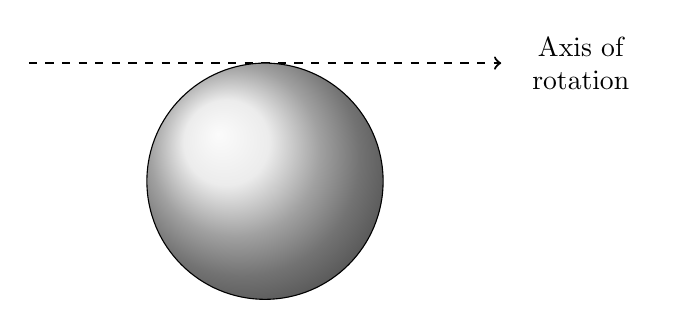
\begin{tikzpicture}
        \draw[thick,dashed,->] (-3,0) -- (3,0) node[anchor=west,text width=5em,text centered] {Axis of rotation};
        \draw[shading=ball,ball color=white!90!black] (0,-1.5) circle (1.5);
    \end{tikzpicture}
    \end{center}
    The moment of inertia of the sphere about this axis is:
    \begin{multicols}{3}
    \begin{choices}
        \wrongchoice{$\dfrac{2}{5} MR^2$}
        \wrongchoice{$\dfrac{2}{3} MR^2$}
        \wrongchoice{$\dfrac{5}{7} MR^2$}
      \correctchoice{$\dfrac{7}{5} MR^2$}
        \wrongchoice{$\dfrac{3}{2} MR^2$}
    \end{choices}
    \end{multicols}
\end{question}
}

\element{serway-mc}{
\begin{question}{serway-ch10-q58}
    A uniform cylinder of radius $R$, mass $M$, and length $L$ rotates freely about a horizontal axis parallel and tangent to the cylinder, as shown below. 
    \begin{center}
    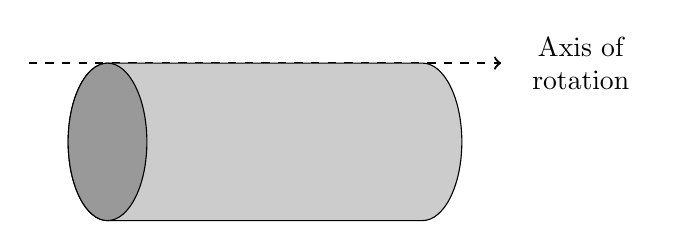
\begin{tikzpicture}
        \draw[thick,dashed,->] (-3,0) -- (3,0) node[anchor=west,text width=5em,text centered] {Axis of rotation};
        \draw[fill=white!80!black] (-2,0) -- (2,0) arc(90:-90:0.5cm and 1cm) -- (-2,-2) arc (270:90:0.5cm and 1cm) --cycle;
        \draw[fill=white!60!black] (-2,-1) circle (0.5cm and 1cm);
    \end{tikzpicture}
    \end{center}
    The moment of inertia of the cylinder about this axis is:
    \begin{multicols}{3}
    \begin{choices}
        \wrongchoice{$\dfrac{1}{2} MR^2$}
        \wrongchoice{$\dfrac{2}{3} MR^2$}
        \wrongchoice{$ MR^2$}
      \correctchoice{$\dfrac{3}{2} MR^2$}
        \wrongchoice{$\dfrac{7}{5} MR^2$}
    \end{choices}
    \end{multicols}
\end{question}
}

\element{serway-mc}{
\begin{question}{serway-ch10-q59}
    The angular speed of the minute hand of a clock, in \si{\radian\per\second}, is:
    \begin{multicols}{3}
    \begin{choices}
        \wrongchoice{$\dfrac{1}{1800} \pi$}
        \wrongchoice{$\dfrac{1}{60} \pi$}
      \correctchoice{$\dfrac{1}{30} \pi$}
        \wrongchoice{$ \pi$}
        \wrongchoice{$120 \pi$}
    \end{choices}
    \end{multicols}
\end{question}
}

\element{serway-mc}{
\begin{question}{serway-ch10-q60}
    The angular speed of the hour hand of a clock, in \si{\radian\per\second}, is:
    \begin{multicols}{3}
    \begin{choices}
        \wrongchoice{$\dfrac{1}{7200} \pi$}
      \correctchoice{$\dfrac{1}{1800} \pi$}
        \wrongchoice{$\dfrac{1}{30} \pi$}
        \wrongchoice{$1800 \pi$}
        \wrongchoice{$7200 \pi$}
    \end{choices}
    \end{multicols}
\end{question}
}

\element{serway-mc}{
\begin{question}{serway-ch10-q61}
    The angular speed of the hour hand of a clock, in \si{\radian\per\minute}, is:
    \begin{multicols}{3}
    \begin{choices}
        \wrongchoice{$\dfrac{1}{1800} \pi$}
        \wrongchoice{$\dfrac{1}{60} \pi$}
      \correctchoice{$\dfrac{1}{30} \pi$}
        \wrongchoice{$ \pi$}
        \wrongchoice{$120 \pi$}
    \end{choices}
    \end{multicols}
\end{question}
}

\newcommand{\serwayChTenQSixtyTwo}{
\begin{tikzpicture}
    \begin{axis}[
        axis y line=left,
        axis x line=middle,
        axis line style={->},
        xlabel={$t$},
        x label style={
            at={(current axis.right of origin)},
            anchor=west,
        },
        x unit=\si{\minute},
        xtick={0,4,8,12,16},
        minor x tick num=1,
        ylabel={$\omega$},
        y label style={
            at={(current axis.above origin)},
            anchor=south,
            rotate=270,
        },
        y unit=\si{\radian\per\second},
        ytick={-2,-1,0,1,2,3},
        yticklabels={$-4\pi$,$-2\pi$,$0$,$2\pi$,$4\pi$,$6\pi$},
        grid=major,
        xmin=0,xmax=17,
        ymin=-2.5,ymax=3.5,
        width=0.8\columnwidth,
        height=0.5\columnwidth,
    ]
    \addplot[line width=1pt,mark=\empty] coordinates { (0,2) (6,2) (10,-2) (16,-2) };
    \end{axis}
\end{tikzpicture}
}

\element{serway-mc}{
\begin{question}{serway-ch10-q62}
    The figure below shows a graph of angular velocity versus time for a man bicycling around a circular track.
    \begin{center}
        \serwayChTenQSixtyTwo
    \end{center}
    What is his average angular acceleration,
        in \si{\radian\per\second\squared},
        in the first 10 minutes?
    \begin{multicols}{3}
    \begin{choices}
        \wrongchoice{zero}
        \wrongchoice{$-\dfrac{\pi}{150}$}
      \correctchoice{$-\dfrac{\pi}{75}$}
        \wrongchoice{$\dfrac{\pi}{75}$}
        \wrongchoice{$\dfrac{\pi}{150}$}
    \end{choices}
    \end{multicols}
\end{question}
}

\element{serway-mc}{
\begin{question}{serway-ch10-q63}
    The figure below shows a graph of angular velocity versus time for a man bicycling around a circular track. 
    \begin{center}
        \serwayChTenQSixtyTwo
    \end{center}
    What is his average angular acceleration, in \si{\radian\per\second\squared},
        in the period from $t=\SI{6}{\minute}$ to $t=\SI{8}{\minute}$?
    \begin{multicols}{3}
    \begin{choices}
        \wrongchoice{zero}
        \wrongchoice{$-\dfrac{\pi}{90}$}
      \correctchoice{$-\dfrac{\pi}{30}$}
        \wrongchoice{$+\dfrac{\pi}{30}$}
        \wrongchoice{$+\dfrac{\pi}{90}$}
    \end{choices}
    \end{multicols}
\end{question}
}

\element{serway-mc}{
\begin{question}{serway-ch10-q64}
    Which of the following diagrams shows a non-zero net torque and a zero net force? 
    All the rods, of length $2r$,
        rotate about an axis that is perpendicular to the rod and fixed in the center of the rod. 
    All the forces are of magnitude $F$ or $2F$ and all distances from the axis are $r$ or $r/2$.
    \begin{multicols}{2}
    \begin{choices}
        \AMCboxDimensions{down=-2cm}
        \wrongchoice{
            \begin{tikzpicture}[scale=0.5]
                \draw[dashed,white!80!black] (-2.5,-0.5) rectangle (3.5,8.5);
                \draw (0,0) rectangle (1,8);
                \draw[fill] (0.5,4) circle (3pt);
                \draw[ultra thick,<-] (0,6) -- ++(180:1cm);
                \draw[ultra thick,<-] (1,2) -- ++(0:1);
            \end{tikzpicture}
        }
        \wrongchoice{
            \begin{tikzpicture}[scale=0.5]
                \draw[dashed,white!80!black] (-2.5,-0.5) rectangle (3.5,8.5);
                \draw (0,0) rectangle (1,8);
                \draw[fill] (0.5,4) circle (3pt);
                \draw[ultra thick,<-] (0,8) -- ++(180:1cm);
                \draw[ultra thick,<-] (1,0) -- ++(0:1cm);
            \end{tikzpicture}
        }
        \wrongchoice{
            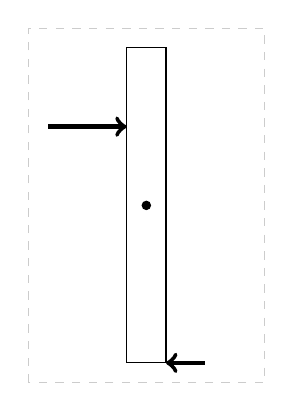
\begin{tikzpicture}[scale=0.5]
                \draw[dashed,white!80!black] (-2.5,-0.5) rectangle (3.5,8.5);
                \draw (0,0) rectangle (1,8);
                \draw[fill] (0.5,4) circle (3pt);
                \draw[ultra thick,<-] (0,6) -- ++(180:2cm);
                \draw[ultra thick,<-] (1,0) -- ++(0:1cm);
            \end{tikzpicture}
        }
        %% ANS is D
        \correctchoice{
            \begin{tikzpicture}[scale=0.5]
                \draw[dashed,white!80!black] (-2.5,-0.5) rectangle (3.5,8.5);
                \draw (0,0) rectangle (1,8);
                \draw[fill] (0.5,4) circle (3pt);
                \draw[ultra thick,<-] (0,6) -- ++(180:1cm);
                \draw[ultra thick,<-] (1,0) -- ++(0:1cm);
            \end{tikzpicture}
        }
        \wrongchoice{
            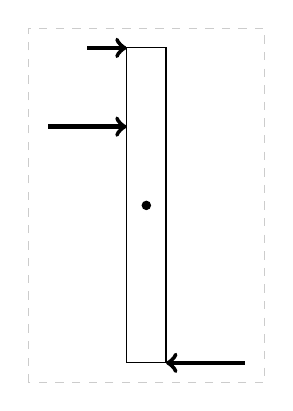
\begin{tikzpicture}[scale=0.5]
                \draw[dashed,white!80!black] (-2.5,-0.5) rectangle (3.5,8.5);
                \draw (0,0) rectangle (1,8);
                \draw[fill] (0.5,4) circle (3pt);
                \draw[ultra thick,<-] (0,8) -- ++(180:1cm);
                \draw[ultra thick,<-] (0,6) -- ++(180:2cm);
                \draw[ultra thick,<-] (1,0) -- ++(0:2cm);
            \end{tikzpicture}
        }
    \end{choices}
    \end{multicols}
\end{question}
}

\element{serway-mc}{
\begin{question}{serway-ch10-q65}
    A small sphere attached to a light rigid rod rotates about an axis perpendicular to and fixed to the other end of the rod. 
    Relative to the positive direction of the axis of rotation,
        the angular positions of the sphere are positive,
        its angular velocity is positive, and its angular acceleration is negative. 
    The sphere is:
    \begin{choices}
        \wrongchoice{rotating clockwise and slowing down.}
      \correctchoice{rotating counterclockwise and slowing down.}
        \wrongchoice{rotating clockwise and speeding up.}
        \wrongchoice{rotating counterclockwise and speeding up.}
        \wrongchoice{first rotating clockwise and then counterclockwise.}
    \end{choices}
\end{question}
}

\element{serway-mc}{
\begin{question}{serway-ch10-q66}
    A small sphere attached to a light rigid rod rotates about an axis perpendicular to and fixed to the other end of the rod. 
    Relative to the positive direction of the axis of rotation,
        the angular positions of the sphere are negative,
        its angular velocity is negative, and its angular acceleration is positive. 
    The sphere is:
    \begin{choices}
      \correctchoice{rotating clockwise and slowing down.}
        \wrongchoice{rotating counterclockwise and slowing down.}
        \wrongchoice{rotating clockwise and speeding up.}
        \wrongchoice{rotating counterclockwise and speeding up.}
        \wrongchoice{first rotating counterclockwise and then clockwise.}
    \end{choices}
\end{question}
}

\element{serway-mc}{
\begin{question}{serway-ch10-q67}
    A small sphere attached to a light rigid rod rotates about an axis perpendicular to and fixed to the other end of the rod. 
    Relative to the positive direction of the axis of rotation,
        the angular positions of the sphere are negative,
        its angular velocity is negative, and its angular acceleration is negative. 
    The sphere is:
    \begin{choices}
        \wrongchoice{rotating clockwise and slowing down.}
        \wrongchoice{rotating counterclockwise and slowing down.}
      \correctchoice{rotating clockwise and speeding up.}
        \wrongchoice{rotating counterclockwise and speeding up.}
        \wrongchoice{first rotating counterclockwise and then clockwise.}
    \end{choices}
\end{question}
}

\newcommand{\serwayChTenQSixtyEight}{
\begin{tikzpicture}
    \begin{axis}[
        axis y line=left,
        axis x line=middle,
        axis line style={->},
        xlabel={time},
        x unit=\si{\second},
        xtick={0,1,2,3,4,5,6,7},
        %ylabel={angular acceleration},
        ylabel={$\alpha$},
        y unit=\si{\radian\per\second\squared},
        ytick={0,2,4,6,8,10},
        grid=major,
        xmin=0,xmax=7.2,
        ymin=0,ymax=10,
        width=0.8\columnwidth,
        height=0.5\columnwidth,
    ]
    \addplot[line width=1pt,mark=\empty] coordinates { (0,3) (4,3) (7,9) };
    \end{axis}
\end{tikzpicture}
}

\element{serway-mc}{
\begin{question}{serway-ch10-q68}
    The graph below shows a plot of angular velocity in \si{\radian\per\second} versus time in \si{\second} from $t=\SI{0}{\second}$ to $t=\SI{7}{\second}$.
    \begin{center}
        \serwayChTenQSixtyEight
    \end{center}
    The change in angular position, $\Delta\theta$,
        during the \SI{7}{\second} period is:
    \begin{multicols}{2}
    \begin{choices}
        \wrongchoice{\SI{21}{\radian}, CW.}
        \wrongchoice{\SI{21}{\radian}, CCW.}
        \wrongchoice{\SI{30}{\radian}, CW.}
      \correctchoice{\SI{30}{\radian}, CCW.}
        \wrongchoice{\SI{39}{\radian}, CCW.}
    \end{choices}
    \end{multicols}
\end{question}
}

\element{serway-mc}{
\begin{question}{serway-ch10-q69}
    The graph below shows a plot of angular velocity in \si{\radian\per\second} versus time in \si{\second} from $t=\SI{0}{\second}$ to $t=\SI{7}{\second}$.
    \begin{center}
        \serwayChTenQSixtyEight
    \end{center}
    The angular position, $\theta$, at $t=\SI{0}{\second}$ is \SI{3.0}{\radian}, clockwise. 
    The angular position, $\theta$, at $t=\SI{7}{\second}$ is:
    \begin{multicols}{2}
    \begin{choices}
        \wrongchoice{\SI{27}{\radian}, CW.}
      \correctchoice{\SI{27}{\radian}, CCW.}
        \wrongchoice{\SI{33}{\radian}, CW.}
        \wrongchoice{\SI{33}{\radian}, CCW.}
        \wrongchoice{\SI{36}{\radian}, CCW.}
    \end{choices}
    \end{multicols}
\end{question}
}

\newcommand{\serwayChTenQSeventy}{
\begin{tikzpicture}
    \begin{axis}[
        axis y line=left,
        axis x line=middle,
        axis line style={->},
        xlabel={time},
        x unit=\si{\second},
        xtick={0,2,4,6,8},
        ylabel={$\alpha$},
        y unit=\si{\radian\per\second\squared},
        ytick={-6,-4,-2,0,2,4},
        grid=major,
        xmin=0,xmax=8.2,
        ymin=-7,ymax=5,
        width=0.8\columnwidth,
        height=0.5\columnwidth,
    ]
    \addplot[line width=1pt,mark=\empty] coordinates { (0,4) (5,-6) (8,-6) };
    \end{axis}
\end{tikzpicture}
}

\element{serway-mc}{
\begin{question}{serway-ch10-q70}
    The graph below shows a plot of angular acceleration versus time
        from $t=\SI{0}{\second}$ to $t=\SI{8}{\second}$. 
    \begin{center}
        \serwayChTenQSeventy
    \end{center}
    The change in angular velocity, $\Delta\omega$,
        during this \SI{8}{\second} period is:
    \begin{multicols}{2}
    \begin{choices}
        \wrongchoice{\SI{18}{\radian\per\second}, CW.}
        \wrongchoice{\SI{18}{\radian\per\second}, CCW.}
      \correctchoice{\SI{23}{\radian\per\second}, CW.}
        \wrongchoice{\SI{23}{\radian\per\second}, CCW.}
        \wrongchoice{\SI{31}{\radian\per\second}, CW.}
    \end{choices}
    \end{multicols}
\end{question}
}

\element{serway-mc}{
\begin{question}{serway-ch10-q71}
    When a wheel is rolling without slipping,
        the magnitude of its velocity relative to the ground is greatest at:
    \begin{choices}
        \wrongchoice{the point in contact with the ground.}
        \wrongchoice{the point at the center of the wheel.}
      \correctchoice{the point at the top of the wheel opposite to the point in contact with the ground.}
        \wrongchoice{the point farthest forward from the center of mass of the wheel.}
        \wrongchoice{the point farthest behind the center of mass of the wheel.}
    \end{choices}
\end{question}
}

\element{serway-mc}{
\begin{question}{serway-ch10-q72}
    The graph below shows a plot of angular acceleration versus time
        from $t=\SI{0}{\second}$ to $t=\SI{8}{\second}$. 
    \begin{center}
        \serwayChTenQSeventy
    \end{center}
    The angular velocity at $t=\SI{0}{\second}$ is $\omega_0=\SI{5}{\radian\per\second}$, CCW.
    The angular velocity, $\omega$, at $t=\SI{8}{\second}$ is:
    \begin{multicols}{2}
    \begin{choices}
      \correctchoice{\SI{11}{\radian\per\second}, CW.}
        \wrongchoice{\SI{11}{\radian\per\second}, CCW.}
        \wrongchoice{\SI{23}{\radian\per\second}, CW.}
        \wrongchoice{\SI{23}{\radian\per\second}, CCW.}
        \wrongchoice{\SI{43}{\radian\per\second}, CW.}
    \end{choices}
    \end{multicols}
\end{question}
}

\element{serway-mc}{
\begin{questionmult}{serway-ch10-q73}
    A rigid rod of length rotates about an axis perpendicular to the rod,
        with one end of the rod fixed to the axis. 
    Which of the following are equal at all points on the rod?
    \begin{choices}
      \correctchoice{the angular position}
      \correctchoice{the angular velocity}
      \correctchoice{the angular acceleration}
        \wrongchoice{the centripetal acceleration}
        \wrongchoice{the tangential acceleration}
        %A: I and II
        %ANS B: I, II, and III
        %C: I, II, III and IV
        %D: I, II, III, IV and V
        %E: I, II and IV.
    \end{choices}
\end{questionmult}
}

\element{serway-mc}{
\begin{question}{serway-ch10-q74}
    When the sum of the external forces and the sum of the external torques on a body are both zero,
        we can conclude that:
    \begin{choices}
        \wrongchoice{the body is moving at constant velocity but is not rotating.}
        \wrongchoice{the body is rotating at constant angular velocity but has no linear velocity.}
        \wrongchoice{the body has neither linear nor angular velocity.}
        \wrongchoice{the body may have constant linear or angular velocity, but not both simultaneously.}
      \correctchoice{the body may have constant linear or constant angular velocity, or both simultaneously.}
    \end{choices}
\end{question}
}

\element{serway-mc}{
\begin{question}{serway-ch10-q75}
    When the center of a bicycle wheel has linear velocity $\vec{v}_{CM}$ relative to the ground,
    \begin{center}
    \begin{tikzpicture}
        %% Ground
        \draw (-3,0) -- (3,0);
        \node[anchor=north,fill,pattern=north east lines,minimum width=6cm, minimum height=0.05cm] at (0,0) {};
        %% Circle
        \draw[thick] (0,1) circle (1cm);
        \draw[fill] (0,1) circle (2pt);
        \draw[fill] (0,2) circle (2pt) node[anchor=south] {$P^{\prime}$};
        \draw[very thick,->] (0,1) -- ++(0:2cm) node[pos=0.9,anchor=south] {$\vec{v}_{CM}$};
    \end{tikzpicture}
    \end{center}
        the velocity relative to the ground of point $P^{\prime}$ at the top of the wheel is:
    \begin{multicols}{3}
    \begin{choices}
        \wrongchoice{zero}
        \wrongchoice{$\vec{v}_{CM}$}
      \correctchoice{$2\vec{v}_{CM}$}
        \wrongchoice{$-\vec{v}_{CM}$}
        \wrongchoice{$-2\vec{v}_{CM}$}
    \end{choices}
    \end{multicols}
\end{question}
}


\endinput


